\begin{tikzpicture}[
    station/.style={red,very thick}
]
    \pgfmathsetlengthmacro{\ssize}{5pt};

    \node[anchor=south west, inner sep=0, opacity=.5] (image) at (0,0) {
        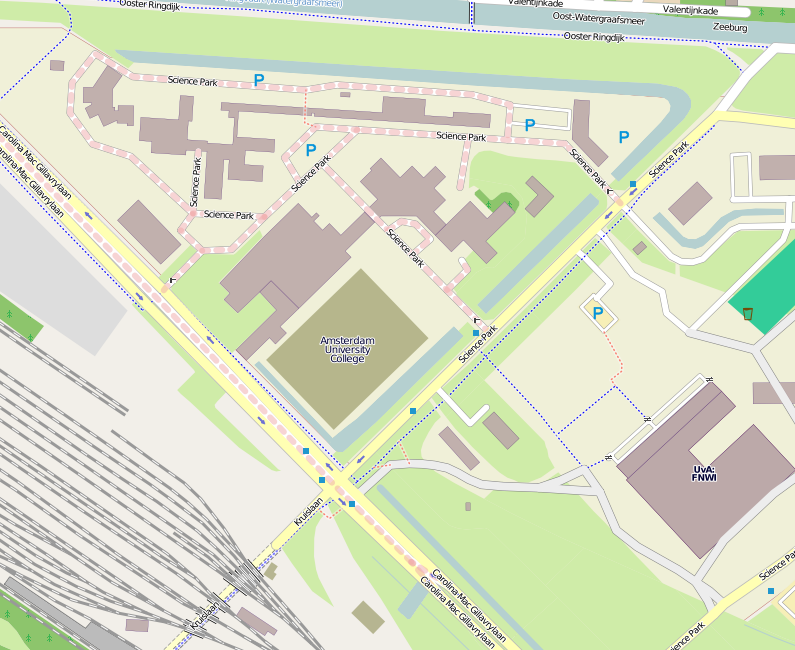
\includegraphics[width=.67\linewidth]{figures/map-sciencepark}
    };

    \begin{scope}[x=(image.south east), y=(image.north west),
                  shift={(-0.005, 0)}]
        \draw[station] (0.3748, 0.5825) circle (\ssize);
        \draw[station] (0.3100, 0.4594) circle (\ssize);
        \draw[station] (0.5950, 0.6533) circle (\ssize);
        \draw[station] (0.7389, 0.8363) circle (\ssize);
        \draw[station] (0.1422, 0.8537) circle (\ssize);
        \draw[station] (0.4986, 0.8358) circle (\ssize);
        \draw[station] (0.8697, 0.3117) circle (\ssize);
    \end{scope}
\end{tikzpicture}
